\chapter{Spectrum processing}
\label{cha:Spectrum}

Spectrum tile in the top menu offers various options for spectrum analysis and presentation. The "Update plot" option is primarily for manually refreshing the canvas when it doesn't update automatically, which should be uncommon but possible. If such an issue arises, kindly report it via the "About/Report bug" option or the main GitHub repository.

\section{Spectrum compare}

The spectrum comparison feature primarily serves the visual comparison of different spectra. It allows for comparing spectra measured under different conditions and samples, and even with different spectroscopes, since each spectrum is loaded with its own loader.

\begin{figure}[H]
    \centering
    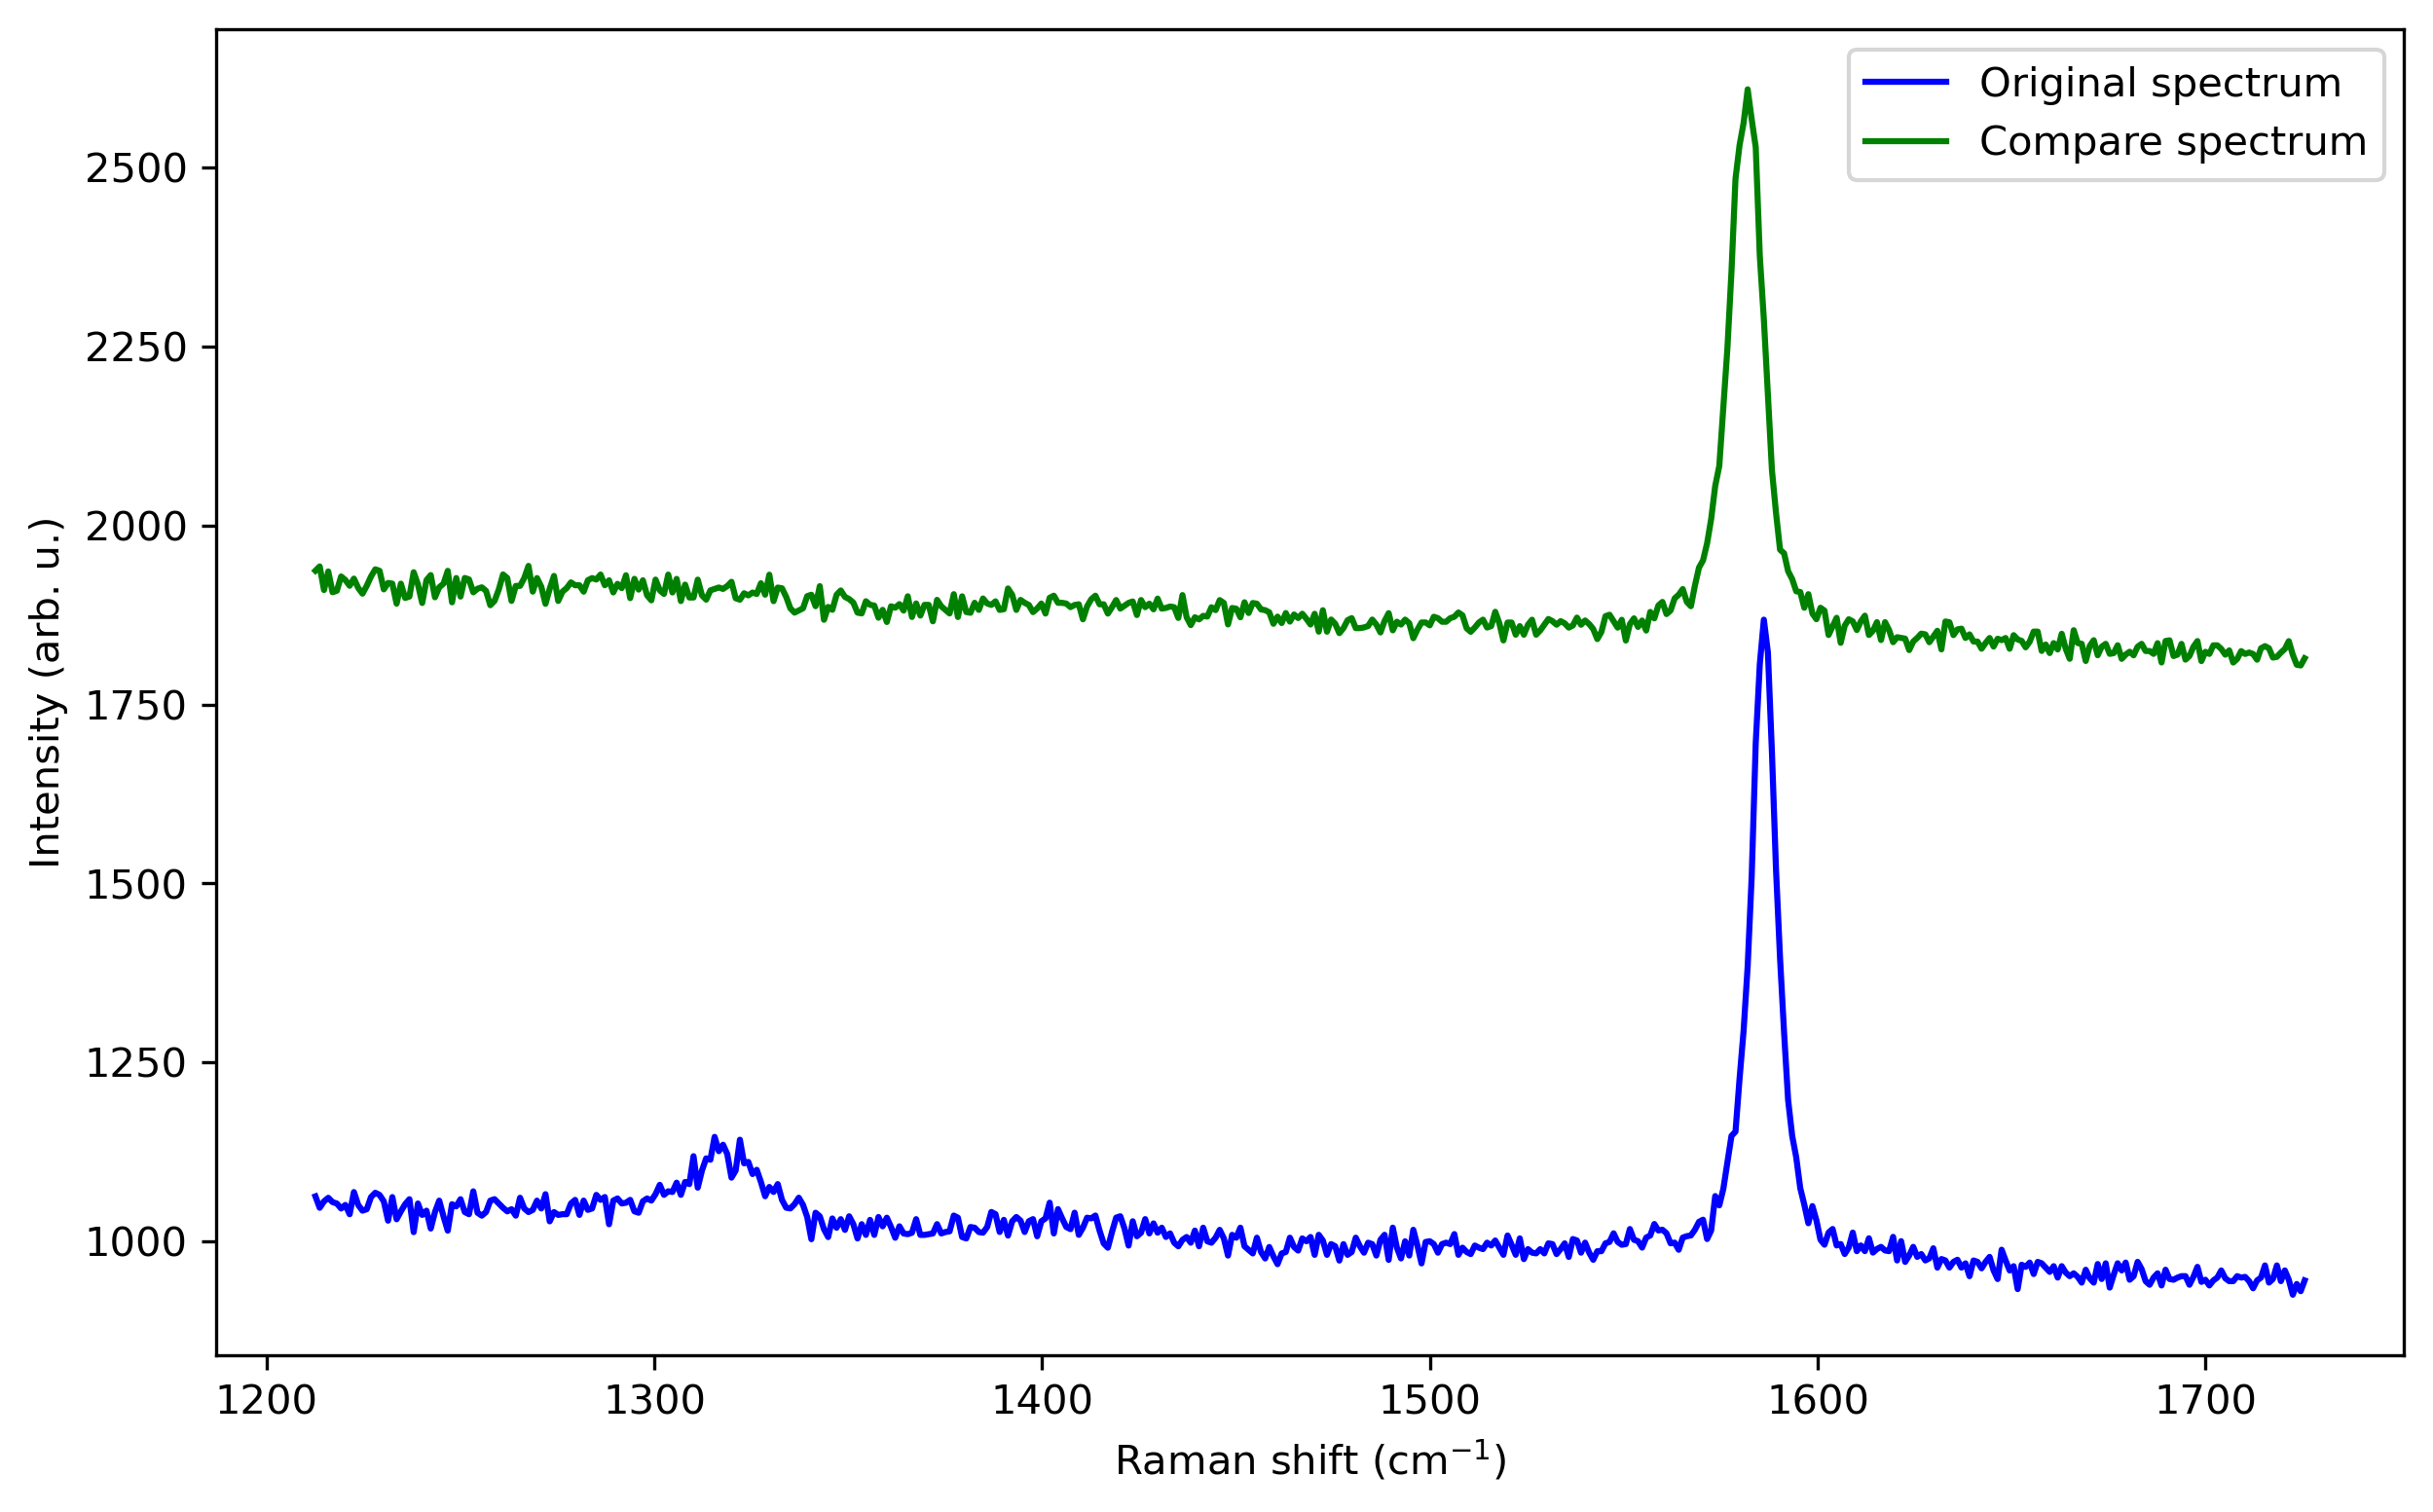
\includegraphics[width=0.8\linewidth]{Resources/Compare.png}
    \caption{Example of spectrum comparison}
    \label{compare}
\end{figure}

Activating the "Compare spectrum" option and selecting a file results in a green overlay plot on the main canvas. While the compared spectrum is loaded, all other features remain enabled, except that analysis (aside from data filtering) will focus exclusively on the main spectrum. To remove it, choose the "Delete compare" option. Figure \ref{compare} illustrates the possible results of the spectrum comparison.

\section{Signal filtering}

To reduce noise and enhance the interpretability of spectral data, the application offers several filtering methods. Each filter has its own characteristics and is suitable for different types of data and noise profiles. For the application of the filter to the data, simply select the type of filter you wish to apply, input the filter parameters, and click "Apply"; this filter will be automatically applied to all data plotted in the Main window. To deactivate the filter, the "Disable" button needs to be clicked.

\begin{figure}[H]
    \centering
    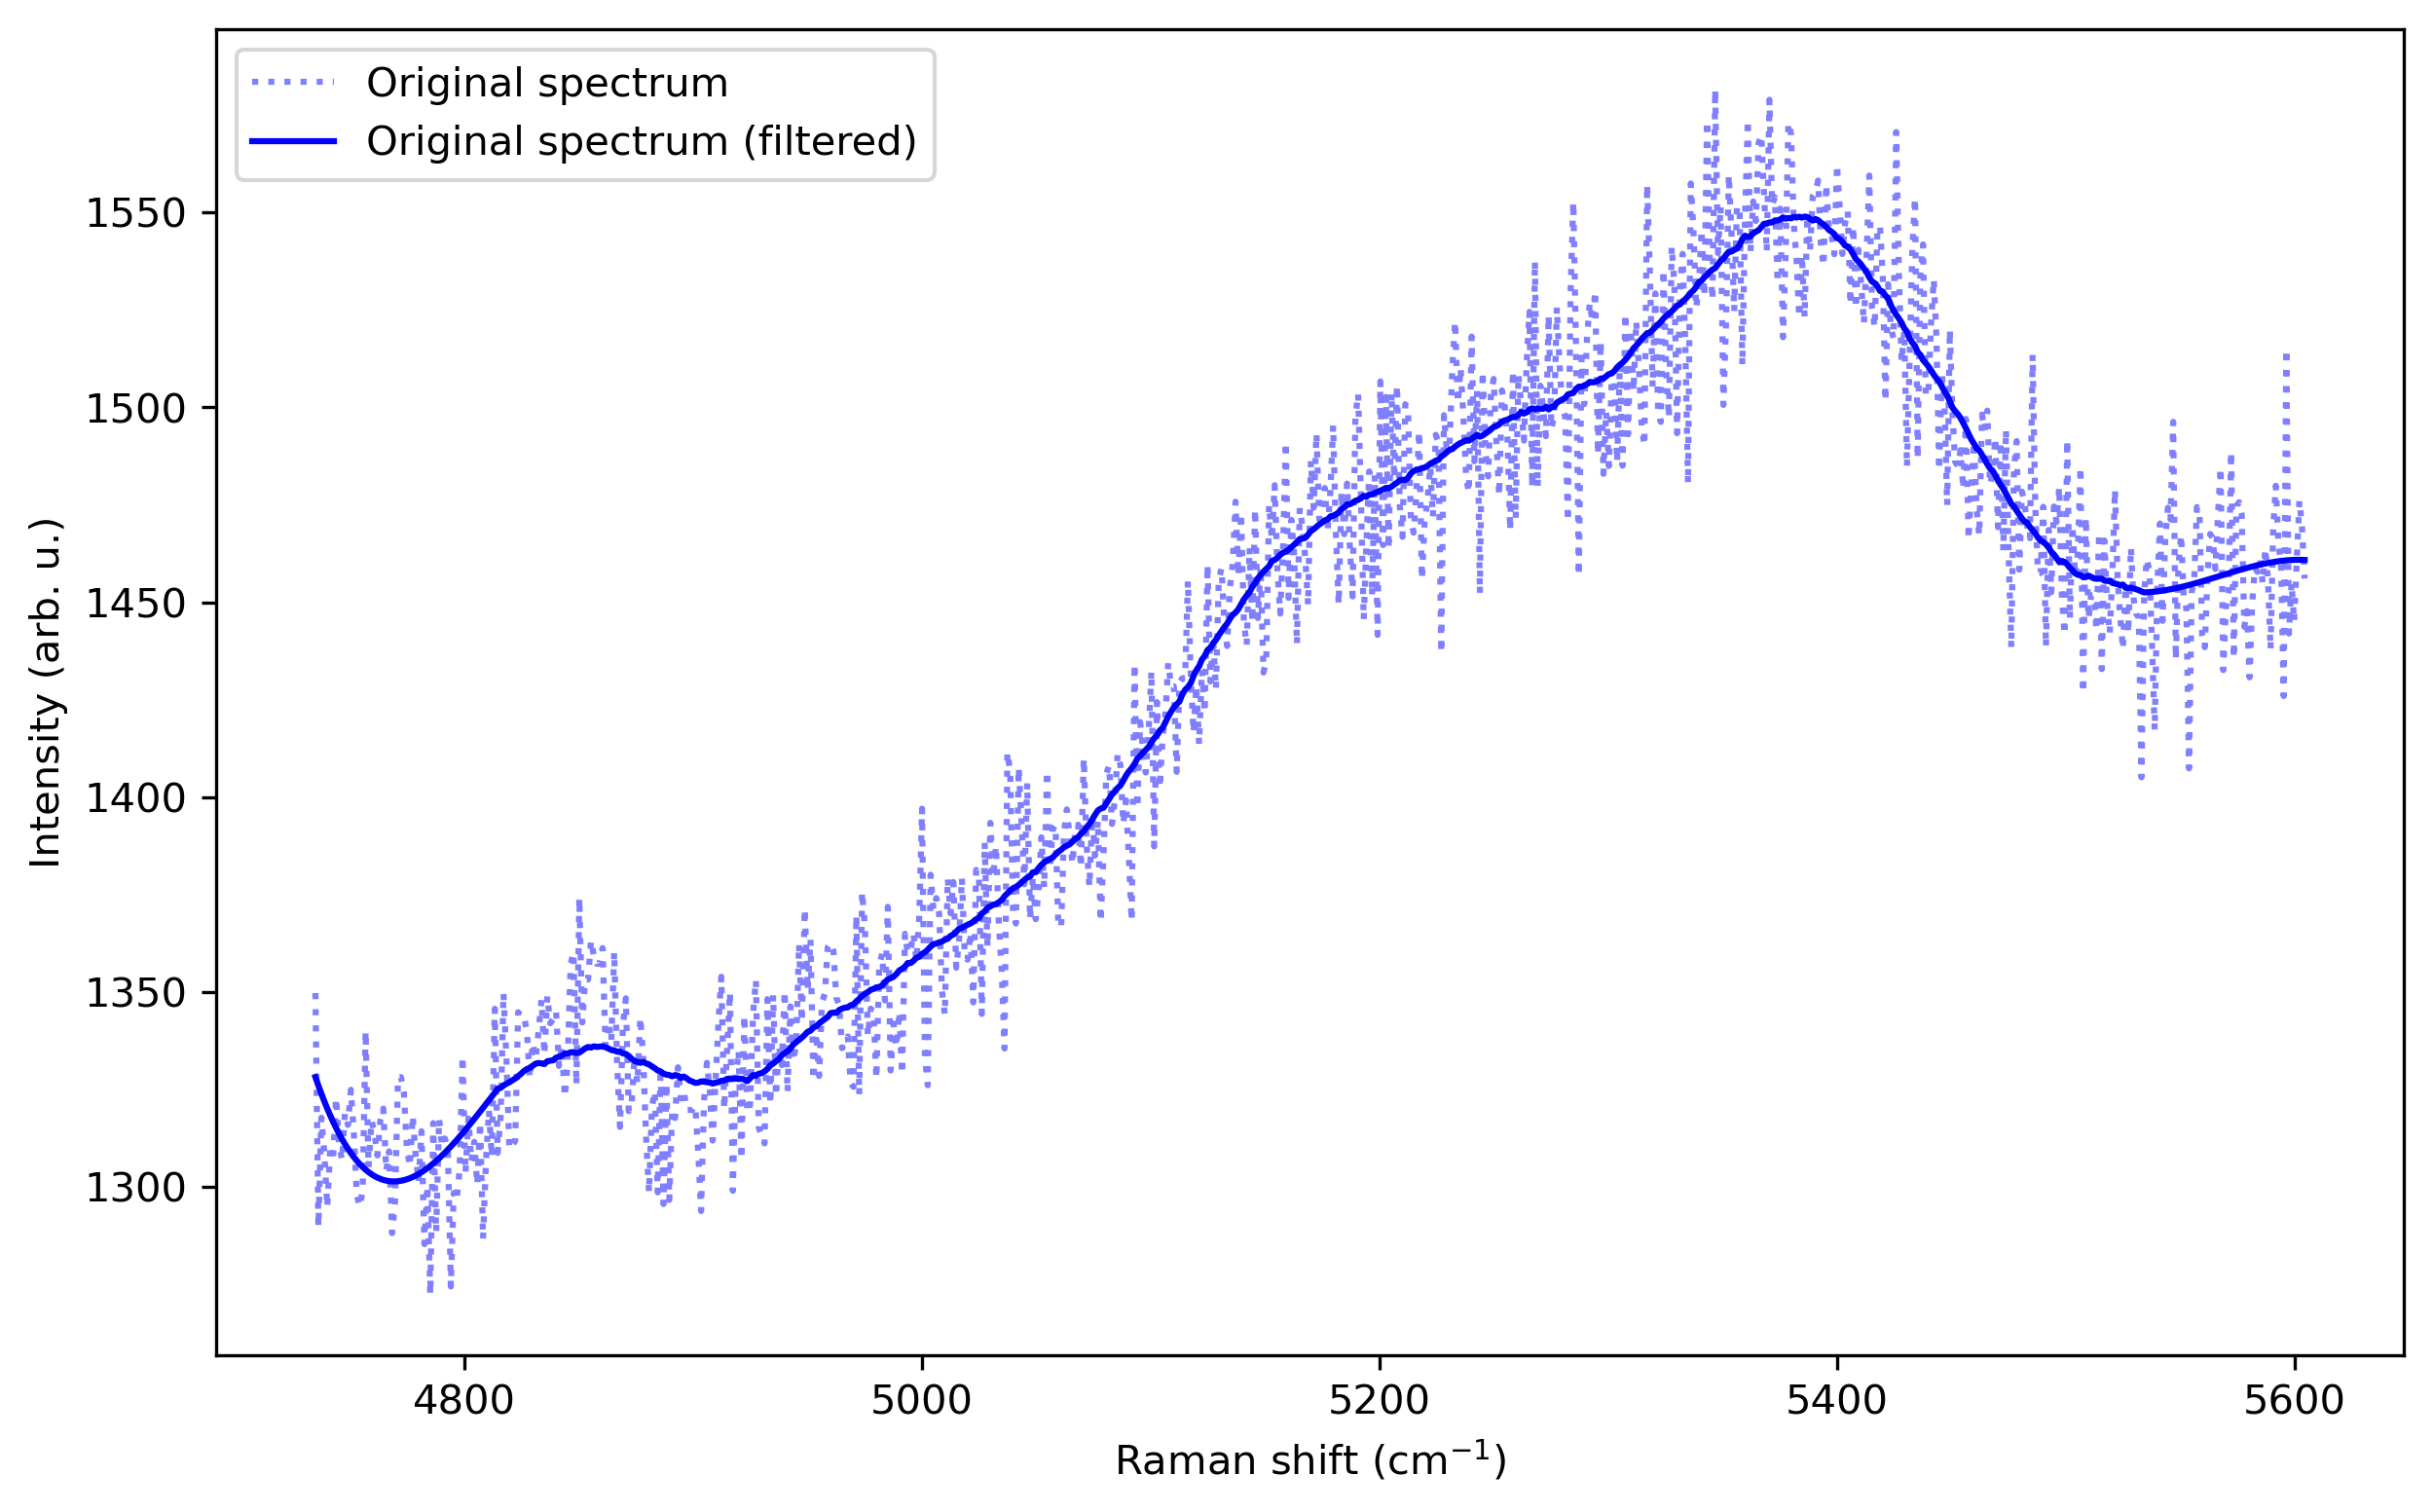
\includegraphics[width=0.75\linewidth]{Resources/filter.png}
    \caption{Example of Savitzky-Golay filter applied on the noisy data}
    \label{filter}
\end{figure}

\subsection{Savitzky–Golay Filter}

The Savitzky–Golay filter smooths data by fitting a low-degree polynomial to a moving window of points using least squares. Unlike a simple moving average, it preserves the original shape and features of the signal, such as peak height and width.

\textbf{Parameters:}
\begin{itemize}
    \item \texttt{window length} – Number of points in the smoothing window. Must be odd and larger than the polynomial order.
    \item \texttt{polyorder} – Order of the polynomial used for fitting (e.g., 2 for quadratic, 3 for cubic).
\end{itemize}

\textbf{Pros:}
\begin{itemize}
    \item Retains peak shapes and derivatives.
    \item Effective in reducing random noise without distorting the signal structure.
\end{itemize}

\textbf{Cons:}
\begin{itemize}
    \item Sensitive to window size; too large a window can flatten peaks.
    \item May introduce artifacts at the edges.
\end{itemize}

\textbf{Recommended Use:}  
Ideal for general-purpose smoothing when the signal shape must be preserved (e.g., Raman or IR spectra).

\textbf{Avoid If:}  
The signal has sharp spikes or highly irregular noise; consider median filtering instead.

\subsection{Moving Average Filter}

The moving average (boxcar) filter replaces each point with the mean of its surrounding neighbors, effectively smoothing high-frequency noise.

\textbf{Parameters:}
\begin{itemize}
    \item \texttt{window\_size} – Width of the averaging window in the number of points.
\end{itemize}

\textbf{Pros:}
\begin{itemize}
    \item Simple and fast to compute.
    \item Smooths out random fluctuations effectively.
\end{itemize}

\textbf{Cons:}
\begin{itemize}
    \item Can blunt sharp features and reduce resolution.
    \item Distorts peak height and width.
\end{itemize}

\textbf{Recommended Use:}  
Suitable for baseline smoothing or reducing random noise when precise peak shapes are not critical.

\textbf{Avoid If:}  
The data contains closely spaced or narrow peaks that must be preserved accurately.

\subsection{Median Filter}

The median filter replaces each point with the median of the surrounding window, making it very effective at removing sharp outliers (e.g., cosmic rays or spikes).

\textbf{Parameters:}
\begin{itemize}
    \item \texttt{window\_size} – Width of the median window. Must be an odd integer.
\end{itemize}

\textbf{Pros:}
\begin{itemize}
    \item Excellent for removing impulsive noise (spikes).
    \item Preserves edges better than moving average.
\end{itemize}

\textbf{Cons:}
\begin{itemize}
    \item Not ideal for reducing continuous Gaussian noise.
    \item Can distort small peaks if the window is too large.
\end{itemize}

\textbf{Recommended Use:}  
Use when data contains discrete spike artifacts or experimental glitches.

\textbf{Avoid If:}  
Your data has small-amplitude features that could be suppressed by the median operation.

\subsection{Fourier Low-Pass Filter}

This method filters the signal in the frequency domain by removing high-frequency components above a specified cutoff. It is suitable for uniformly spaced data.

\textbf{Parameters:}
\begin{itemize}
    \item \texttt{cutoff} – Cutoff frequency (in units of inverse x-axis units), above which components are removed.
\end{itemize}

\textbf{Pros:}
\begin{itemize}
    \item Effective for removing high-frequency noise.
    \item Retains the overall spectral shape well.
\end{itemize}

\textbf{Cons:}
\begin{itemize}
    \item Requires uniformly spaced data.
    \item Can introduce ringing artifacts (Gibbs phenomenon).
\end{itemize}

\textbf{Recommended Use:}  
Effective when noise is dominated by high-frequency components and the data are evenly spaced.

\textbf{Avoid If:}  
The data is unevenly sampled, or if phase preservation is critical (e.g., for derivative spectroscopy).

\section{Spectral subtraction}

There are several operations that could be performed with the spectrum before the analysis itself. Such preprocessing steps can often help reduce model complexity and enhance the comparability of results between different fits.

\subsection{Minimum subtraction}

Spectral data often contain an artificial offset to prevent the detection system from returning negative intensity. This simple function subtracts the minimum intensity value (y axis) from the whole dataset and sets the lowest point to zero.

\subsection{Linear subtraction}

Linear subtraction calculates the slope of the data from the first and last display points and then subtracts this slope from the displayed data.

\subsection{Spectrum subtraction}

This feature will allow the user to subtract the entire spectrum file from the displayed spectrum. In cases where the spectra have different ranges and varying point densities, the subtraction will be performed only at the overlapping spectra, and the spectrum with lower point density will be used as the grid on which the other spectrum will be interpolated.

\section{Spectrum normalization}

This function allows the user to normalize the spectrum according to the selected range in the data. It uses the same logic as data zoom; instead of focusing on the selected range, it normalizes the displayed spectrum to the maximum amplitude in that range.

\section{Batch spectrum processing}

The single spectrum processing does not overwrite the original data files, but the user has the option to save them manually using the "Save spectrum" option. Performing the preprocessing steps in batch (more data files together) requires different options. All of the preprocessing techniques mentioned above could be performed in batch; the user just needs to define the input folder (the folder where the data on which the preprocessing step will be performed is located) and the output folder (where to save the data after the preprocessing step). It is done by two consecutive dialog windows, which makes it user friendly. To distinguish between the original and modified data, the modified data are saved with the same filename and extension corresponding to the preprocessing step that was performed (for example, subtraction of the minimum = *original filename*\_sub\_min.txt. The data are saved in the Default format, so they can later be loaded into the ASS easily with the "Load function" or with the "Ctrl+d" shortcut.

Since the normalization logic also needs the operating range on which the normalization will be performed, it is triggered even before setting the input and output folders through dialog windows.

\section{Spectrum configuration}
The final option in the "Spectrum" menu lets users customize details of the rendered image, including the plot title, axis labels, data labels, and the dataset comparison offset. These features enable plot customization according to user preferences and allow shifting the app's focus from Raman to other spectroscopy techniques by simply changing axis labels, as the analysis workflow remains consistent. Once these changes are applied, they stay in the apps settings even after the restart.

\begin{figure}[H]
    \centering
    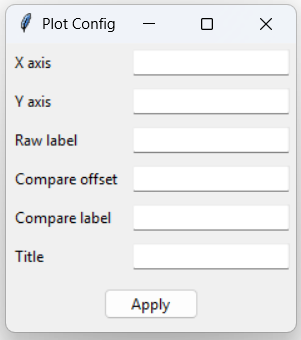
\includegraphics[width=0.4\linewidth]{Resources/plot_config.png}
    \caption{Plot configuration window}
    \label{plot_config}
\end{figure}